\documentclass[10pt]{exam}
\usepackage[phy]{template-for-exam}
\usepackage{tikz, graphicx, multicol}

\title{Acoustical Phenomena}
\author{Rohrbach}
\date{\today}

\begin{document}
\maketitle

\begin{questions}

\uplevel{\section*{Doppler Effect (\emph{review})}}

\question
  You are in a convertible traveling at 45 m/s.  The car in front of you is only traveling at 30 m/s.  It has a broken muffler and emits a sound with a frequency of 200 Hz.  What frequency do you hear? \vs[3]


\uplevel{\section*{Resonance}}

\question
  Define the following terms:

  \begin{parts}
    \part natural frequency \vs 
    \part resonance \vs 
  \end{parts}

\question
  Explain how resonance relates to a kid on a swing. \vs[2]

\question
  Explain how the Mythbusters used the concept of resonance to shatter the glass. \vs[2]

\question
  Why was Jaime Vendera flicking the glass before he sang at it? \vs[2]

\pagebreak



\uplevel{\section*{Beats}}

\question
  What are ``\emph{beats}''? \vs

\question
  What has to be true about the two tones that are being sounded together in order for beats to occur? \vs


\question
  Look at the diagram below (Figure 20.21 from the textbook).  Label the regions of constructive and destructive interference.

  \begin{tikzpicture}
    \node at (0,0) 
      {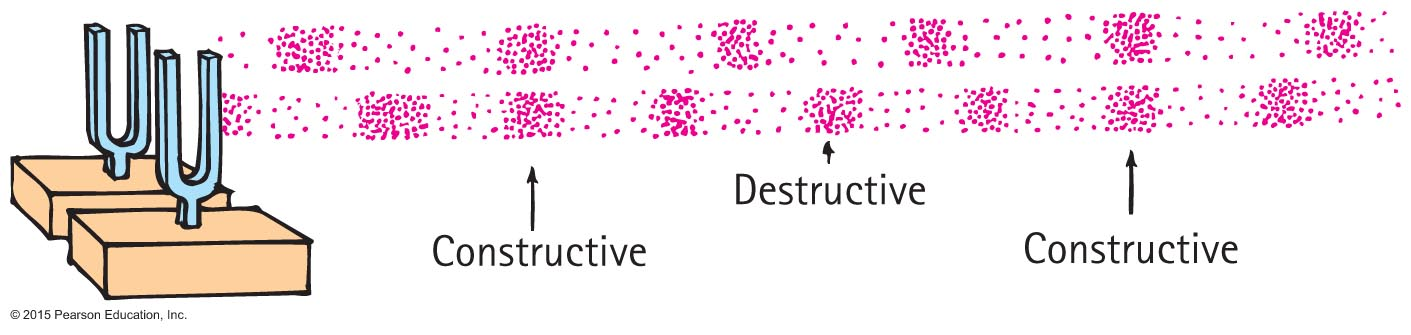
\includegraphics[width=12cm]{Fig20_21.jpg}};
    \fill[white] (-3,-1) rectangle (6,.26);
  \end{tikzpicture}

  \question
  Take a look at the illustration below that refers to a wave of frequency 10 Hz being played at the same time as a wave of frequency 12 Hz.

  \vspace{-1em}

  \begin{multicols}{2}
    \centering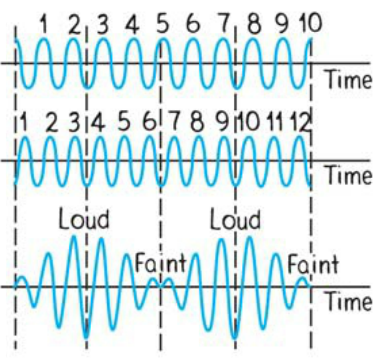
\includegraphics[width=6cm]{Figure.png}

    \begin{parts}
      \part Label the regions of constructive and destructive interference.
      \part What is the frequency of the tone being produced? \vs
      \part What is the beat frequency? \vs
    \end{parts}
  \end{multicols}
 
\question
  Draw your own beats!  Draw two bugs jumping on the water.  One bug jumps forward 3 cm each hop; the other bug jumps forward 4 cm each hop.

  \begin{tikzpicture}
    \draw[dotted] (0,0) grid[step=0.5] (15,-1.5);
  \end{tikzpicture}


\question Using all that we've talked about, come up with your own description of the cause of beats. \vs



\end{questions}

\end{document}